\section{Related Work and Motivation}\label{sec:background} 


In this section, we discuss related work about automated code completion to situate the problems and present a motivating analysis.  

\subsection{Code Completion}
Code completion is a task to suggest the next code token from a given context. More formally, given a sequence of $m$ tokens $x_1 ... x_m$ as a context, code completion aims to predict the next $n$ tokens to complete a sentence $x_1 ... x_{m+n}$. 
The learning objective of a language model for code completion is to minimize a conditional probability distribution of the following function:
% standard language modelling objective that applied to code completion is a conditional probability distribution $P$ as follow:

\[ P(x_{1:m+n}) = \prod_{i=1}^{m+n} P(x_i|x_1 ... x_{i-1}) \]

% There are several approaches proposed for code completion. 
% Starting from the traditional tools by listing out all the possible attributes or methods that can invoke, heuristic rules~\cite{hou2010towards}, program history~\cite{robbes2008program}, and code examples~\cite{bruch2009learning}.

\textbf{Statistical language models.} Previously, several studies proposed code completion approaches using various types of techniques (e.g., heuristic, statistical, and deep learning).
Heuristic-based approaches aim to recommend source code based on rules~\cite{hou2010towards}, program history~\cite{robbes2008program}, and code examples~\cite{bruch2009learning}.
However, heuristic-based approaches are heavily based on rules and patterns that researchers need to develop, which is time-consuming and expensive.
Therefore, statistical language models have been proposed to automatically learn the naturalness of source code based on a probabilistic of the occurrence of source code.
For example, Hindle~\ea~\cite{10.5555/2337223.2337322, hindle2016naturalness} argued that source code is natural and repetitive (similar to natural language) and found that an n-gram approach can accurately predict the next code token based on a given context.
Raychev~\ea~\cite{raychev2016probabilistic} proposed TGEN, a probabilistic-based learning approach with decision tree structures.
However, the statistical language models are able to learn only the limited number of $n$ consecutive tokens (according to the $n$-gram algorithm), which does not reflect the nature of the source code that is usually long (i.e., long-term dependencies).



% Then there are statistical language models to capture the statistical patterns in source code using the occurrence probabilities of sequence of words such as n-gram~\cite{hindle2016naturalness} and decision tree~\cite{raychev2016probabilistic}. 


% Traditionally, code completion is formulated as a probabilistic language model (e.g., n-gram~\cite{hindle2016naturalness}) where the goal is to suggest the next probable code tokens based on a given context of the existing sequence of source code.
% To address various limitations of the traditional probabilistic language models (e.g., \kla{??}), 

% \kla{Gam will do the rest.}
% \kla{need to do this para with Wannita}

% together with the similar characteristic to natural language, code completion is shaped to Natural Language Processing (NLP) problem.
 % in Natural Language Processing (NLP)
 % The model is designed specially to solve the code completion Out-of-Vocabulary (OOV) problem.

\textbf{LSTM-based language models.} To address the limitation of the statistical language models, Long Short-Term Memory (LSTM)-based deep learning approaches are applied to the code completion task.
However, existing LSTM-based language models can only learn the semantic information of the source code, without considering its syntactic structure.
Thus, to ensure that the LSTM-based code completion models recognize the syntactic information, Abstract Syntax Tree (AST) is widely used by the previous work.
For example, Li~\ea~\cite{li2017code} proposed Pointer Mixture Networks, which is an LSTM-based architecture for predicting the AST node. 
Similarly, Svyatkovskiy~\ea~\cite{svyatkovskiy2019pythia} proposed Pythia, which is an LSTM-based approach that incorporates ASTs information through the Word2Vec embedding approach.
While such RNN-based and LSTM-based are able to handle longer sequences of source code than statistical language models, the approach remain inaccurate due to the sequential nature of source code processing, the limited ability to capture long-term dependencies, and the limited ability to recognize the importance of different code tokens.


% Additionally, together with a more complex model, the data such as ASTs information has also been introduced to train the model on syntactical structures of source codes.
% Nonetheless, the early state of deep learning architectures still consider the weight parameters of each token equally which in fact some source code tokens may be less or more important.
% can recognize longer sequences  by recursively inputting the previous output state to the current step. \kla{out of context}
% Next after code completion is shaped to \gls{nlp} problem. There are the coming of deep learning for code completion. The deep neural networks such as RNNs and LSTMs are applied.

\textbf{Transformer-based language models.} 
To address the limitations of LSTM-based language models, the Transformer architecture is introduced for the code completion task.
% Particularly, with the attention mechanism~\cite{vaswani2017attention} inside the Transformer architecture, the model is able to  differentiate the importance of code tokens, allowing the models to pay attention to only the important tokens, not the less important ones.
Generally, the development of Transformer-based language models consists of two steps: pre-training and fine-tuning.
Pre-training is a process to train a Transformer-based language model in a self-supervised manner (i.e., without labels), allowing the language models to self-understand given data by itself (i.e., natural language or programming languages).
Normally, the language models for code completion are trained using a Causal Language Model (CLM) (i.e., predicting the unknown token after a sequence of known tokens).
Once a language model is pre-trained, the model is then fine-tuned on a specific dataset (e.g., PY150~\cite{raychev2016probabilistic}) with the same learning objective as the pre-training process (i.e., CLM).
For example, Lu~\ea~\cite{lu2021codexglue} proposed CodeGPT-based models, which is based on a GPT-2 architecture~\cite{radford2019language} that is pre-trained on both Natural Language (NL) corpus (i.e., WebText) and/or Programming Language (PL) corpus (i.e., CodeSearchNet)---i.e., PL only for CodeGPT, and NL+PL for CodeGPT-adapt.

% from Microsoft Research proposed
To ensure that the Transformer-based language models recognize the syntactic structure of source code, Kim~\ea~proposed TravTrans~\cite{kim2021code}, a vanilla Transformer-based language model that incorporates ASTs information through different encoding styles.
Similarly, Wang~\ea~\cite{wang2021code} leverages AST information with a vanilla Transformer-based language model, but using a different AST encoding technique (i.e., by flattening the ASTs nodes).
However, these AST-based code completion approaches also leverage AST information at the inference phase, which requires source code to be completed at the inference time so the AST information can be parsed and obtained from the source code. 
Therefore, in practice, source code is often incomplete and not compilable (e.g., syntax errors), making the existing AST-based code completion approaches not applicable in real-world scenarios.



% Wang~\ea~\cite{wang2021code}

% the AST information 

% Some work apply flattened ASTs as Graphs then untilize with attention architectures~.


% many representation of ASTs in TravTrans~\cite{kim2021code}, a Transformers-based model to predict AST nodes.


% Not only code sequences but ASTs also still be utilized with Transformers in many works.

% Some work apply flattened ASTs as Graphs then untilize with attention architectures~\cite{wang2021code}.
% Last but not least, currently one of the most powerful generative model is GPT-3~\cite{brown2020language} or Codex~\cite{chen2021evaluating} in software engineering field, however; there are little knowledge on the architecture and training methods in public.




% CodeGPT and CodeGPT-adapt~\cite{lu2021codexglue} are also build up from the same architecture of GPT-2 but are pre-trained on source code dataset (CodeSearchNet).



% variants of the generative pre-train transformers model have been presented, for instance, GPT-2~\cite{radford2019language} is pre-trained from English natural language dataset (WebText) and use to fine-tune on source code.




%and propose SynComp in this work.

% \textit{finish} \kla{end with limitations}


% \subsection{Text Generation Decoding Methods}
% The open-ended text generation is to generate text from the given context. 

% \kla{We may need to provide background: problem/task formulation (token/line)? how code completion is different from other tasks? (the language head?) what is the multi-task learning?}

\begin{figure}[h]
    \centering
    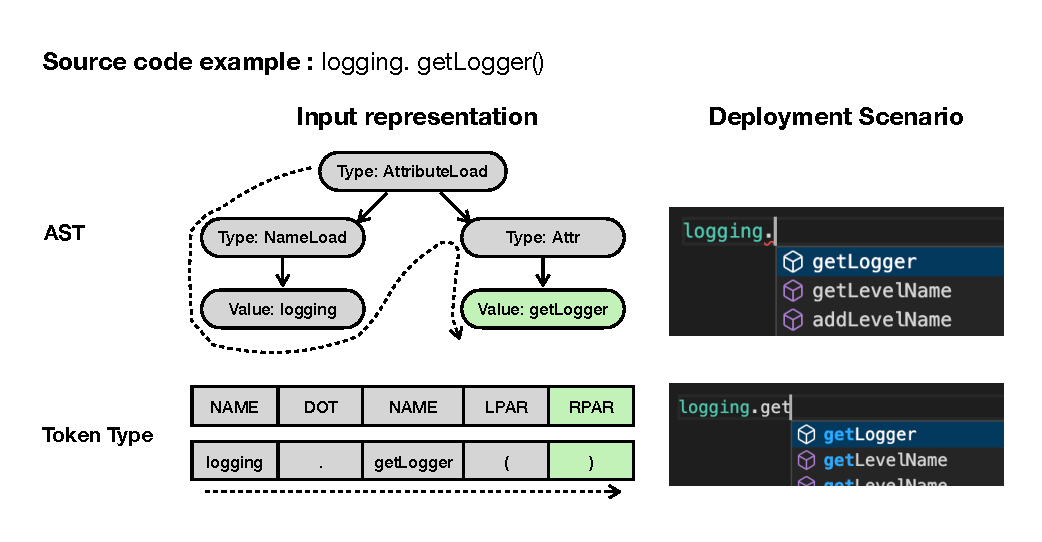
\includegraphics[width=\columnwidth]{figures/motivation.pdf}
    \caption{The comparison between AST and Token Type representations and the ideal deployment scenarios.}
    \label{fig:motivation}
\end{figure}

\subsection{A Motivating Example}

% In this section, we illustrate the limitation of an AST-based code completion approach through a motivating example followed by a motivating analysis.


% \kla{explain the analysis / parsable here / and present the findings. along with Figure 1 and new Figure on the results?}

% In this section, we conduct the analysis to prove the statement that ASTs information is not \emph{on-the-fly} information, i.e. in real-world scenario of code completion task, ASTs information is likely to be unable to extract which lead to the unseemliness of automate code completion.

% In this section, we explain our motivation of this paper.
% There are 2 main motivations: the AST node representation is not a natural order for code prediction, and the AST extraction require the complete and syntactically correct source code as inputs.
% Firstly, 

% \textbf{A Motivating Example.} 
Let's consider a code snippet \texttt{logging.getLogger()} as an example (see Figure~\ref{fig:motivation}).
\texttt{logging.} is the input code token, while \texttt{getLogger()} is the code token to be predicted.
Below, we illustrate two key limitations of the AST-based code completion approach by using TravTrans~\cite{kim2021code} as an example, which makes the existing AST-based code completion \emph{not able to predict next code tokens on-the-fly}.

\emph{First,} the learning objective of TravTrans does not reflect the natural order of typing source code sequences.
Since representing the source code as AST node sequence by traversing the AST, the order of the node sequence are inconsistent with the token sequence~\cite{liu2022unified}.
For example, at the learning phase, TravTrans~\cite{kim2021code} represents the input code tokens as a sequence of an AST node structurekl (i.e., [\texttt{AttributeLoad}, \texttt{NameLoad}, \texttt{logging}, \texttt{Attr}]) in order to predict the next AST node (i.e., [\texttt{getLogger}]).
However, this learning objective does not mimic the natural sequence of code tokens (i.e., [\texttt{logging}, \texttt{.}, \texttt{getLogger}, \texttt{(}, \texttt{)}]), meaning that the programming language-specific characters (e.g., dot [\texttt{.}] and parenthesis [\texttt{(},~\texttt{)}]) are currently ignored.
Therefore, in many cases at the deployment scenarios, such AST node information needs to be post-processed in order to successfully perform code completion in practice (e.g., add missing tokens [\texttt{(},~\texttt{)}], convert [\texttt{Attr}] to [\texttt{.}]).

% With this learning objective, TravTrans requires AST information to be available in order to perform a code completion task.
% This manual post-processing step is also required for other AST-based code completion approaches (e.g., CodeFill by Izadi~\ea~\cite{izadi2022codefill}).
% Unfortunately, this post-processing step remains manual.

% These require the developers' effort to type the missing tokens and/or special post-processing process to convert the nodes back to the source code.
% For example, let's consider the input code token \texttt{logging.} in Figure~\ref{fig:motivation}, TravTrans~\cite{kim2021code} will leverage the \texttt{ast.parse} function provided by the Python AST library to generate the AST node structure for the given input token (i.e., the grey nodes)
% Like in this example, \texttt{logging.} is considered as an AttributeLoad, which consists of two parts, i.e., NameLoad and Attribute.


% The input representation in Fig.~\ref{fig:motivation} shows an example of AST information in TravTrans~\cite{kim2021code} which is represented in node structure.
% TravTrans predicts codes by traversal via AST node in depth-first-search order.
% This kind of node structure is abstract and not the natural order of source code comparing to the code that developers type.

% predicting a sequence of AST nodes (i.e., given a sequence of [AttributeLoad, NameLoad, logging, Attr], then predicting [getLogger])---which does not reflect the natural order of the code sequences that a code completion approach should predict (i.e., given a sequence of [logging.], then predicting [getLogger()]).


% realistic.....

% More specifically, the AST representation in the example has no \emph{dot} and \emph{parenthesis} ( \emph{.} , \emph{(} , \emph{)} ) characters, but \emph{NameLoad} and \emph{Attr} nodes instead.



% These require the developers' effort to type the missing tokens and/or special post-processing process to convert the nodes back to the source code.


\emph{Second,} in order to use AST information as an input, TravTrans~\cite{kim2021code} requires source code to be completed at the inference time so the AST information can be parsed and obtained from the source code. 
For example, in Figure~\ref{fig:motivation}, if developers type \texttt{logging.}, TravTrans can successfully recommend the next token (e.g., \texttt{getLogger)}).
However, source code is often incomplete and not compilable.
For example, in Figure~\ref{fig:motivation}, if developers type \texttt{logging.get}, TravTrans cannot correctly recommend the next token, due to the syntax errors during the AST parsing step.


\subsection{A Motivating Analysis}
\label{sec:motivation}

% \textbf{Motivating Analysis.} 
To demonstrate the significance of the problem of the AST-based code completion approaches, we perform a motivating analysis to investigate how often AST information could be provided at the inference phase, making AST-based code completion can be executed at the inference phase.

% \textbf{Approach.} 
Let's assume that a developer is typing a Python program character-by-character, we aim to analyze how often an AST parser can/cannot successfully parse a Python program at each character.
To do so, we select a statistical representative sample of 383 syntactically correct Python files from the PY150 dataset (with a confidence level of 95\% and a confidence interval of 5\%).\footnote{https://www.surveysystem.com/sscalc.htm}
Since we simulate the application of AST-based code completion at the character level, we execute a Python AST parser\footnote{https://docs.python.org/3/library/ast.html} at each character incrementally.
In total, we execute a Python AST parser for 1,263,296 times according to the total of 1,263,296 characters.
We find that 33.96\% of the executions can be successfully parsed, while 66.04\% of the executions fail to parse due to syntax errors.



\begin{table}[h]
    \centering
    \begin{tabular}{c|c}
        AST Parsable? & Percentage \\
        \hline
        Successful executions & 33.96\% \\
        Failed executions & 66.04\%
        % Success & 28.68\% \\
        % Syntax Error & 71.32\%
    \end{tabular}
    \caption{The percentage of the successful/failed executions of the Python AST parser from the 1,263,296 executions.}
    \label{tab:simulation}
\end{table}

\begin{tcolorbox}
\emph{\textbf{Finding:} For every two out of three characters that developers type, AST-based code completion cannot be performed at all due to the failed execution of the Python AST parser, limiting its ability to perform code completion on-the-fly at the inference time.
Since existing syntax-aware code completion is not on-the-fly and existing on-the-fly code completion is not syntax-aware, this paper aims to address these significant gaps by proposing a syntactic-aware on-the-fly Python code completion approach.
}
\end{tcolorbox}

% While existing syntax-aware 
% }This finding highlights the need for syntactic-aware on-the-fly code completion---that is not yet available.





% Then, we incrementally add one character at a time and parse each time step to AST parser~\footnote{https://docs.python.org/3/library/ast.html}.
% As a result, we receive 1,263,296  typing-simulation timesteps in total.



% we attempt to simulate the real-world scenario that developers are typing the source code character-by-character and count the total results of the successful AST extraction.
% This shows how does AST extracting process perform for the inputs during code completion.



% Moreover, we conduct an analysis to study the AST parsing rate in practice.
% In other word, we attempt to simulate the real-world scenario that developers are typing the source code character-by-character and count the total results of the successful AST extraction.
% This shows how does AST extracting process perform for the inputs during code completion.

% \textbf{Approach.} To simulate the use-case of code completion in practice, we first randomly select 383 python files from PY150 dataset (section 4.1).
% These sample size should allow us to generalize the conclusion about the ratio of ASTs parsing rate to all files with a confidence level of 95\% and a confidence interval of 5\%\footnote{https://www.surveysystem.com/sscalc.htm}.
% Next, normally in coding process (i.e. code completion scenario) the developers type the code character by character.
% Next, to simulate the typing pattern, we split these files into a character-level.
% The special characters (e.g. $\langle EOL \rangle$) are treated as one character.
% Then, we incrementally add one character at a time and parse each time step to AST parser~\footnote{https://docs.python.org/3/library/ast.html}.
% As a result, we receive 1,263,296  typing-simulation timesteps in total.
% Then, we create the typing pattern dataset by sequentially add one character at a time to a new data point.
% As a result, we receive 1,542,810 typing-simulation data points in total.
% Then we parse all data points to ASTs parser using python AST library~\footnote{https://docs.python.org/3/library/ast.html} to find the AST parsing rate for \emph{on-the-fly} scenario.



% \textbf{Results.} \textbf{The AST parser can successfully parse AST }
% Table~\ref{tab:simulation} presents the statistics of the AST parsing rate.
% We find that 




% The result is shown in Table.~\ref{tab:simulation}.
% The number of AST parsing success and error samples are 428,973 and 834,323 respectively, which are represented as 33.96\% and 66.04\% of total samples.
% The number of AST parsing success and error samples are 442,417 and 1,100,393 respectively, which are represented as 28.68\% and 71.32\% of total samples.

% From the simulation results, we can observe that surprisingly most of the time the AST information cannot be extracted.
% More concretely, almost seven out of every ten characters that developers type will fail the AST parsing.
% Not to mention that this is in case of syntactically correct typing only, because our files are from PY150 dataset which has only the syntactically correct files.
% That means in actual cases the successful result of AST parsing rate could be worse than these numbers.

% Therefore, the analysis shows that AST information is not \emph{on-the-fly} information, leading to the limitations of previous works which apply AST information as inputs.
% The example of deployment scenarios in Fig.~\ref{fig:motivation} shows that unlike our token type approach, the AST code completion can only suggest on some positions.
% Such approaches may cause the unseemliness of automate code completion.
% % This also confirms the previous works' limitations, i.e. current code completion approach are either on-the-fly or syntactic-aware but not both.
% % We are motivated by these limitations and propose 
% These findings motivate us and highlights the need for Syntactic-Aware On-the-Fly Code Completion.

